\section{Kommunikationskostenoptimierung}
\hyphenation{High--Per-for-mance}
\hyphenation{Per-for-mance}
\hyphenation{Com-pu-ting}
\hyphenation{Be-rech-nungs-eng-pass}
Das Papier \cite[Kap.3]{mainpaper} beschreibt in seinem dritten Kapitel Strategien zur Reduktion von Kommunikationskosten bei der Umsetzung der 3D-FFT in einer High-Performance Architektur.\\

Die Kommunikation findet im High-Performance Kontext zwischen verschiedenen Prozessen/Prozessoren statt, deren lokale Daten aktualisiert werden m"ussen.\\
Kommunikationskosten sind dabei die verwendeten Aufw"ande in Zeit f"ur Synchronisationsabschnitte zwischen einzelnen Datenverarbeitungsschritten.\\

Durch die Ergebnisse aus dem vorigen Kapitel, in dem verschiedene M"oglichkeiten zur Umsetzung der 3D-FFT auf Grafikprozessoren behandelt werden, wird hier die genauere Betrachtung der Kommunikationskostenoptimierung motiviert.\\

Die durch die Verwendung von GPU's erreichte Beschleunigung durch Parallelismus optimiert alle Programmanteile um ein vielfaches mit der Ausnahme der Kommunikation.\\

\begin{figure}
\centering
  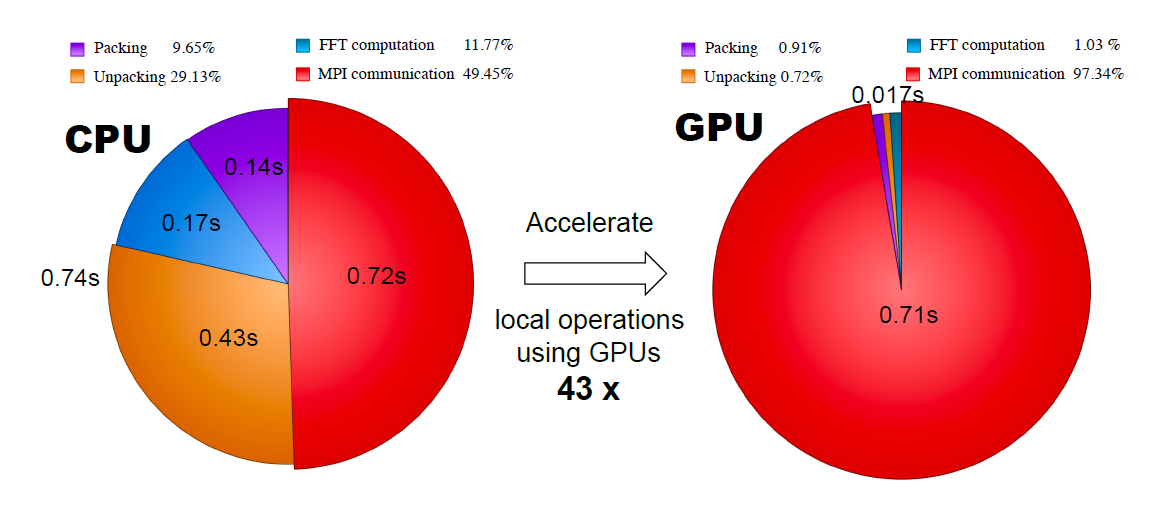
\includegraphics[width=\linewidth]{res/speedup.png}
  \caption{\cite[Abb. 3]{mainpaper} Kreisdiagramme zur Visualisierung von Erfolgen und Bottlenecks bei der GPU Beschleunigung von 3D-FFT's}
  \label{fig:speedup}
\end{figure}

Wie Abbildung \ref{fig:speedup} zeigt hat sich die Zeit, welche im FFT-Algorithmus f"ur Kommunikation zwischen den GPU's/CPU's aufgewendet wird, nur vernachl"assigbar ver"andert. Alle anderen Aktionen (Unpacking, Processing, Packing) haben sich erheblich durch Parallelisierung mit GPUs beschleunigt ($ \frac{0.74s}{0.017s} \approx 43.5$-fache Beschleunigung).\\
\\
Wird Kommunikationszeit mitbetrachtet ist die Beschleunigung $\frac{0.14s+0.17s+0.42s+0.72s}{0.017s+0.71s}=200,8\%$, also nur 2-fach.

Prinzipiell ist Kommunikation ebenfalls parallelisierbar. Da Kommunikation jedoch der Verbreitung einer frisch errechneten, neuen Wahrheit auf anderen Prozessoren dient, h"angt der Grad der Parallelisierbarkeit direkt an der unmittelbaren Wichtigkeit dieser Wahrheit f"ur weitere Berechnungsschritte.\\
Diese Eigenschaft macht Kommunikation hinsichtlich der beteiligten Prozesse oft zu einem inherent seriellen, d.h. in einem gewissen Grad nicht parallelisierbaren Problemanteil.\\
Inherente serielle Anteile in einer Problemstellung limitieren den m"oglichen maximalen Speedup durch Parallelisierung der gesamten Applikation.\\
Diese Sachverhalte k"onnen am FFT-Problem durch die Einteilung in Phasen beobachtet werden. Zwischen jeder Berechnungsphase m"ussen die verwendeten 3D-Tensoren transponiert werden, wodurch neue Werte bei der Werteaufteilung in den Zust"andigkeitsbereich anderer Prozesse fallen und m"ussen daher an diese kommuniziert werden, um die Berechnung fortzuf"uhren.\\
%TODO cite sources
Da Kommunikation unter dem vorgesetzten Ziel der Multi-Prozessorbeschleunigung der Applikation FFT unvermeidbar ist und die Kommunikation selbst zum Berechnungsengpass f"uhrt, muss weiter die Optimierung dieser Kommunikation behandelt werden.


\subsection{Systemarchitektur}

\begin{figure}
\centering
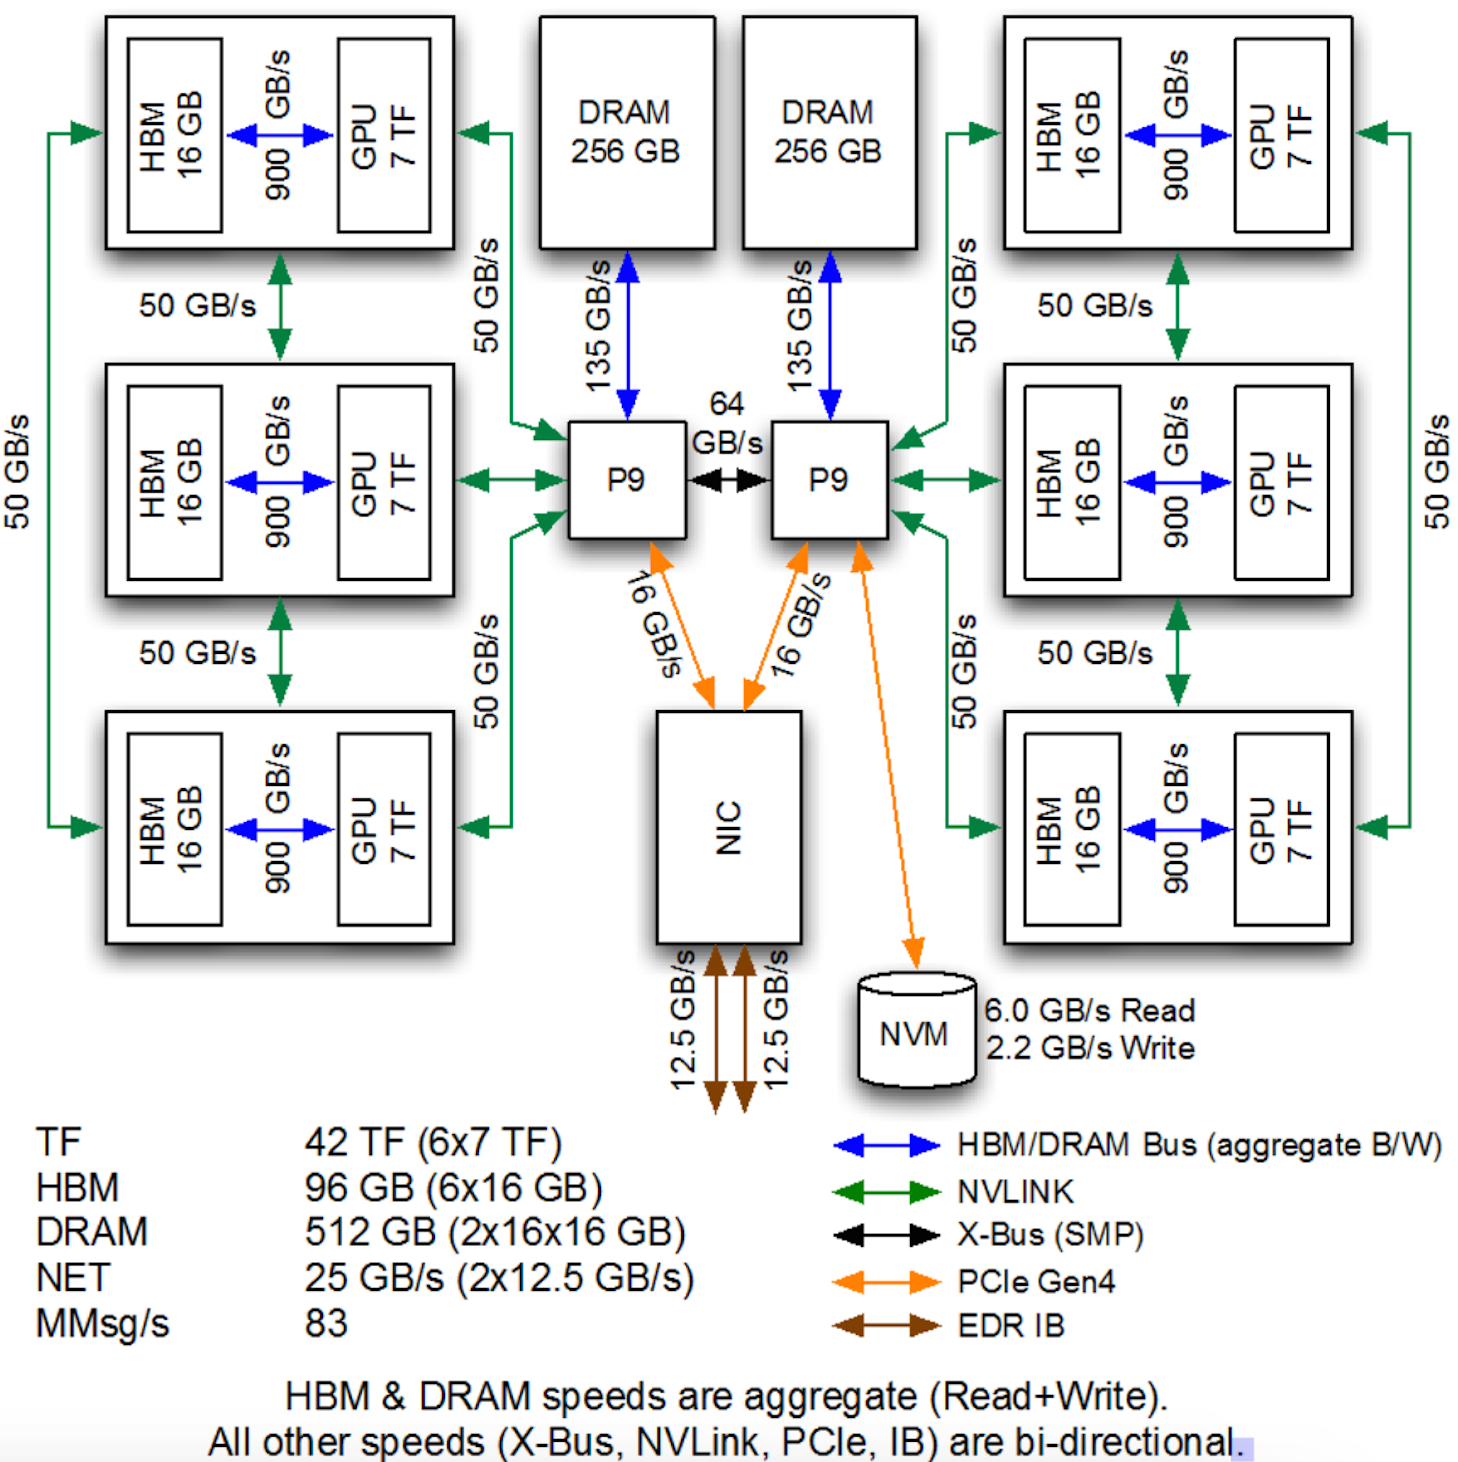
\includegraphics[width=0.6\textwidth]{res/architecture.png}
\caption{\cite[Abb. 1]{mainpaper} Aufbau des Summit Supercomputers, verwendete Kommunikationstechnologien und Komponenten}
	\label{fig:architecture}
\end{figure}

Abbildung \ref{fig:architecture} zeigt die generelle Systemarchitektur des Summit Supercomputers in Oak Ridge National Laboratory(ORNL), zu dem sich die vorgestellten "Uberlegungen im Papier zu relativieren scheinen.\\
Der Summit-Supercomputer im Oak Ridge National Laboratory, Tennessee, ist ein Multi-Prozessor-Supercomputer, der seit 2018 in Betrieb ist. Der Verwendungszweck des Rechners ist der Wissenschaft zugeschrieben.
\\
Der Rechner besitzt 4608 Knoten, welche hybrid mit je 2 CPU's (IBM POWER9) und je 6 GPU's (NVIDIA Volta V100s). Die Knoten sind in einer Non-Blocking Fat Tree Topologie angelegt (vgl. \cite{osummit})\\
\\
Ein Fat-Tree ist eine Topologie, bei der Switches zu einem Bin"arbaum verkn"upft werden. Endknoten, also Prozessoren, werden dabei an den Bl"attern des Baumes plaziert.\\
Ma"sgeblich f"ur den Fat-Tree ist dabei die Regel, dass f"ur jeden Switch im System die Anzahl der Verbindungen nach unten, gleich der Anzahl der Verbindungen nach oben ist, also die eine Elter(n)verbindung gleich viele Verbindungen hat wie beide Kindverbindungen. Daraus folgt die Anzahl der Verbindungen pro switch in abh"angigkeit der Baumh"ohe $h$, maximaler Baumh"ohe $h_{max}$, Der H"ohe am Wurzelknoten $h_{root}=0$ und der Anzahl der Elternverbindung eines Blattknotens $c$ (hier: $c=1$):
\begin{itemize}
	\item Anzahl Elterverbindungen/Kindverbindungen : $(h_{max}+1-h)*c$
	\item Anzahl Verbindungen pro Kind : $\frac{(h_{max}+1-h)*c}{2}$ bei 2 Kindern
\end{itemize}
Die Verbindungsanzahl ist daher maximal am Wurzelknoten mit $h_{max}+1$, der Baum wird nach oben hin \glqq dicker\grqq (\textit{fat}).
H"alt eine Fat-Tree Topologie das Verh"altnis von Eltern- zu Kindverbindung von $1:1$ ein, nennt man diese Non-Blocking. Die Gegenteilige Blocking-Eigenschaft ist bei Nichteinhaltung festzustellen.\\
Ist das Verh"altnis unausgeglichen ist die Kommunikation durch den konkreten unausgeglichenen Switch limitiert. Zum Beispiel k"onnten doppelt so viele Kindverbindungen existieren als Elternverbindungen ($1:2)$. So k"onnen verh"altnism"a"sig viele Kindknoten "uber den Switch zeitgleich kommunizieren, jedoch kann nur die H"alfte aller Kindkommunikation an Eltern weitergereicht werden. Man spricht bei diesem Beispiel von einem Blocking-Faktor von 2, Kind zu Eltern.\\
\\
Die Topologie erreicht durch die das exponentielle Wachstum des Bin"arbaumes mit der Baumtiefe schnell eine gro"se Anzahl verkn"upfbarer Prozessoren. (vgl. \cite{fattree})\\
\\
Die Grafik Abbildung \ref{fig:architecture} zeigt Knoten, welche "uber verschiedene Arten von Networking/Bussen verbunden sind. Diese verschiedenen Networking-Technologien gehen mit verschiedenen "Ubertragungseigenschaften (vorrangig Bandbreite) einher. Ebenfalls zu erkennen is das Konzept eines Sockels (\textit{eng. socket}), welcher mehrere Prozessoren zusammenfasst. 

Alle Prozessoren sind mit dem Sockel Verbunden und dadurch zusammengefasst.
Die NVLINK Technologie erlaubt 2 zus"atzliche (50GB/s) Verbindungen zur Sockelverbindung. Diese Verbindungen sind P2P zu anderen Prozessoren(\cite[FAQ, What is NVLINK?]{osummit})
Mit 8 Prozessoren pro Sockel muss jedoch Sockelintern noch eine andere Topologie als P2P verwendet werden. \cite[Abb. 1]{mainpaper} suggeriert hier eine Ringtopologie.
%TODO check if with NVLINK 50Gb is the speed set for bidirectional communication
Zwischen den Sockeln exisitiert ein X-Bus (64GB/s).
Theoretisch k"onnen also maximal $\frac{64GB/s}{50GB/s} = 1.28$ Prozessoren cross-socket kommunizerien. Unter der Annahme, dass jeder Prozess im Schnitt mit jedem anderen Prozess gleich viel kommuniziert  entstehen demnach Kommunikationsengp"asse zuerst bei der cross-socket Kommunikation.\\
Bestimmte Kommunikationsstrategien verhalten sich also besser auf bestimmten Zielarchitekturen als andere.
\cite{mainpaper} versucht deshalb unter anderem durch Benchmarking bessere L"osungen zu ermitteln. 



\subsection{Relevante Technologien}
\cite{mainpaper} benennt einige verwendete Technologien, gibt jedoch selbst dem Leser oft wenig Kontext zu diesen. Deshalb wird im Folgenden zu diesen Technologien der Kontext hergestellt.

\subsubsection{ NVIDIA GPUDirect }
	ist eine Technologie, die den direkten Zugriff von P"aripherie auf den Speicher von NVIDIA GPU's zul"asst. Dieser Vorgang wird als \textit{Remote Direct Memory Access} bezeichnet (RDMA).
		Dadurch wird der Umweg "uber traditionellen RAM vermieden. Beispiele f"ur P"aripherien sind Netzwerkadapter, Speicher (wie Solid State Drives) und andere Graphikkarten. Es ist letztere Eigenschaft, welche im Kontext des Papiers vorrangig von Bedeutung ist (vgl. \cite{gpud}).

\subsubsection{ \textit{Message Passing Interface} (MPI) }
MPI ist ein Standard, der eine Schnittstelle f"ur Nachrichten zwischen Prozessen spezifiziert. Portabilit"at und Einfachheit werden als prim"are Ziele angegeben (vgl. \cite[Kap. 1.1]{mpi}). Es gibt mehrere Implementierungen dieses Standards, zum Beispiel die Open-Source-Variante OpenMPI (\cite{openmpi}).

In verteilten Systemen wird MPI als Abstraktion f"ur die Kommunikation zwischen parallelen Prozessoren/Prozessen verwendet.

\subsubsection{ CUDA }
Die \textit{\textbf{C}ompute \textbf{U}nified \textbf{D}evice \textbf{A}rchitecture}, entwickelt von NVIDIA ist eine Plattform und Programmiermodell f"ur parallele Berechnungen auf NVIDIA GPUs. 

\subsubsection{ CUDA-aware MPI }
Ist eine Kombination aus CUDA und MPI. Da CUDA mit dem MPI Standard kompatibel ist, sind MPI-Implementierungen durch CUDA m"oglich. Die resultierende MPI-Implementierung ist plattformspezifischer und stellt dadurch in vielen F"allen eine bessere Umsetzung des MPI-Standards auf speziell NVIDIA GPUs dar.

\subsection{Weitere Spezielle Terminologie}
\subsubsection{Sockel \textit{(eng. socket)}}
Ein Sockel fasst im Kontext von \cite{mainpaper} mehrere Prozessoren zusammen. Diese Zusammenfassung verursacht, bedingt durch die Systemarchitektur, spezielle Eigenschaften bei Relationen der Prozessoren untereinander (hier: verf"ugbare Kommunikationstechnologie).\\
Folgende Terminologie wird dabei verwendet:
\begin{defi}[\textit{same-socket-communication}]
Ein Kommunikationsvorgang, welcher zwischen zwei Prozessoren unter dem selben Sockel erfolgt.
\end{defi}
\begin{defi}[\textit{cross-socket-communication}]
Ein Kommunikationsvorgang, welcher zwischen zwei Prozessoren erfolgt, welche sich nicht gemeinsam auf einem Sockel befinden.
\end{defi}

\subsubsection{MPI\_Alltoall}
\textit{MPI\_Alltoall} ist eine Kommunikationsroutine des Message Passing Interfaces. Dabei Senden alle $N$ Prozesse Nachrichten der selben Gr"o"se zu allen $N$ Prozessen (inklusive dem eigenen Prozess). Der Kommunikationsaufwand betr"agt also $N^2 * Nachrichtenl"ange$.\\
Es wird ein Kommunikationspuffer verwendet, dessen Gr"o"se $N*Nachrichtenl"ange$ betr"agt. (vgl. \cite{MPImanpage})\\
Im Papier \cite{mainpaper} scheint eine spezielle Implementierung von MPI\_All2All f"ur den Summit Computer verwendet.

\subsubsection{MPI P2P}
Als Peer to Peer (P2P) Kommunikation bezeichnet man eine Kommunikationsstrategie, bei der alle n"otigen Informationen von einem kommunizierenden Knoten zum anderen direkt, also ohne Umwege, ausgetauscht werden. Dabei sind die Parameter der konkreten Kommunikation prinzipiell an keine weiteren Eigenschaften gebunden.\\
\cite{mainpaper} scheint nicht genau auf die Realisierung dieser Strategie einzugehen. Da der MPI-Standard keine P2P funktion zu definieren scheint, kann an dieser Stelle angenommen werden, dass diese Art der Kommunikation wird wahrscheinlich mit MPI\_Send und MPI\_Recv aufrufen realisiert wird.
Auch hier scheint das Papier \cite{mainpaper} wieder eine spziielle Implementierung f"ur den Summit Computer zu referenzieren.

\subsubsection{Kommunikationsrichtung}
\begin{defi}[Unidirektionale Kommunikation (\textit{ eng. unidirectional communication })]
In einem abgeschlossenen Kommunikationsvorgang zwischen $p1$ und $p2$ werden Daten ausschlie"sslich von $p1$ nach $p2$ kommuniziert.
\end{defi}
\begin{defi}[Bidirektionale Kommunikation (\textit{ eng. bidirectional communication })]
In einem abgeschlossenen Kommunikationsvorgang zwischen $p1$ und $p2$ k"onnen Daten sowohl von $p1$ nach $p2$, als auch von $p2$ nach $p1$ ausgetauscht werden.
\end{defi}

\subsubsection{3D-FFT Datenkomposition}
Der Input der 3D-FFT ist ein 3D-Tensor. Die daraufhin ben"otigten Operationen zu Berechnung der FFT sind abh"angig vom Algorithmus. Jedoch k"onnen durch eine effiziente B"undelung von von einer Operation gemeinsam ben"otigten Information Kommunikationskosten gespart werden.
\cite{mainpaper} verwendet daher folgende Datenkompositionen:
\begin{enumerate}
	\item \textit{pencil}\\
		Dt. Stift, suggeriert einen eindimensional ausgedehnten Anteil am Tensor, also ein 3D Tensor mit einer der Dimensionen $\{1,1,N\},\{1,N,1\},\{N,1,1\}$.
	\item \textit{slab}\\
		Dt. Platte, suggeriert einen zweidimension ausgedehnten Anteil am Tensor, also ein 3D Tensor mit einer der Dimensionen $\{N,N,1\},\{N,1,N\},\{1,N,N\}$.
\end{enumerate}

\subsection{L"osungsans"atze}
Konzeptionell gibt es 2 Optionen um Kommunikationskosten zu verringern.
\begin{itemize}
	\item Option1: Verwendung eines besseren Algorithmus hinsichtlich serieller Anteile und Kommunikation.
	\item Option2: Verbesserung der Kommunikationsstrategie unter Einbeziehung von Eigenschaften der Systemarchitektur.
\end{itemize}

\subsubsection{Ansatz 1}
\cite[Abbildung 4]{mainpaper} zeigt das Ergebnis eines Benchmarking-Versuchs mit dem Verh"altnis von Prozessor-Operationen (in Gflops/s) zu der Anzahl der verwendeten Knoten im Cluster.\\
Verwendete Strategien sind:
\begin{enumerate}
	\item Summit MPI Alltoall
	\item Summit MPI P2P
\end{enumerate}
Die Unterschiede sind nicht Algorithmisch. Die Untersuchung bezieht sich also auf die kommunikativen Eigenschaften der Systemarchitektur (Option 2).\\
Ergebnis: Stategie 2 scheint f"ur geringer als 4 Knotenzahlen besser zu sein, sinkt jedoch sogar nacher weiter ab.
Strategie 1 scheint generell jedoch besser zu skalieren und "ubernimmt bei mehr Knoten stark die F"uhrung. Es ist jedoch erwähnt, dass der Effekt ab 128 Knoten abnimmt, da nicht mehr genügend Parallelisierung für die verwendete Problemgröße vorherrscht.\\
\cite{mainpaper} geht jedoch selbst weiter nicht auf eine m"ogliche Begr"undung ein.\\
Spekulativ ist die Verteilung der Prozessorknoten in der Systemarchitektur verantwortlich. Die n"achstgr"o"sere Anzahl der in der Messung verwendeten Knoten ist 8. Der Summit Supercomputer verwaltet 6 GPU's pro Sockel (vgl. \cite{summit,osummit}), was bei einer ben"otigten Knotenanzahl von 4 Knoten nicht n"otigerweise zu einer cross-socket Kommunikation f"uhrt, welche sich negativ auf das Kommunikationsbild auswirken k"onnte. Bei 8 Knoten wird cross-socket Kommunikation unter der Pr"amisse, dass nur GPU's verwendet werden, jedoch unvermeidbar. Innehalb eines Sockels bietet die Systemarchitektur mehr m"oglichkeiten zur Kommunikation an, was den Unterschied von 4 zu 8 verwendeten Knoten erkl"aren k"onnte.

\subsubsection{Ansatz 2}
\begin{figure}
\centering
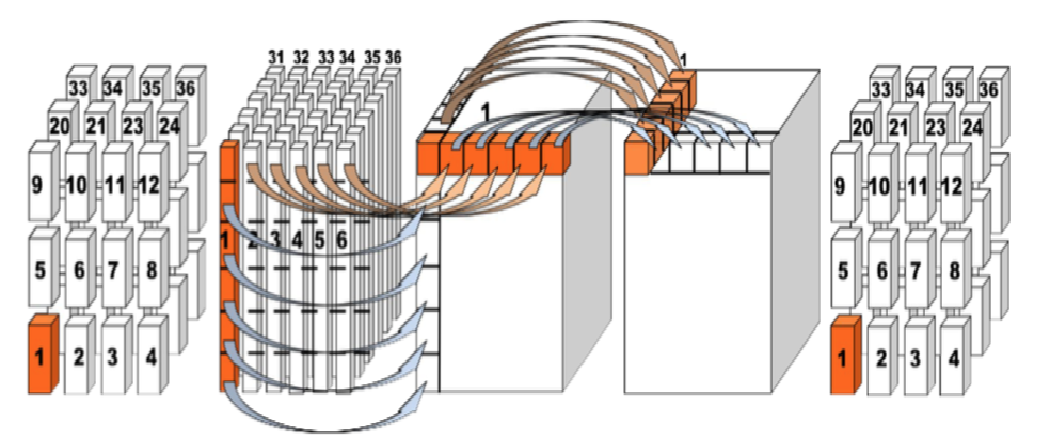
\includegraphics[width=0.6\textwidth]{res/algo.png}
\caption{\cite[Abb. 2]{mainpaper} Prinzipieller Aufbau des 3D-FFT Algorithmus. }
	\label{fig:algo}
\end{figure}

Die Kommunikation kann algorithmisch ge"andert werden (Option 1).\\
Der zuerst vorgestellte Algorithmus agiert in folgenden Phasen:
\begin{enumerate}
	\item Transform X
	\item Transform Y
	\item Transform Z
	\item Move Back to Original
\end{enumerate}
Zwischen den Phasen wird Kommuniziert. Die Kommunikation verh"alt sich zu den jeweiligen Phasen sequenziel, d.h. ist nicht mit einer Phase parallelisierbar, oder f"ahig zu Pipelining.\\
Sichtbar wird dies in Abbildung \ref{fig:algo}.\\
K"onnen die kommunikativen Anteile der Phasen zusammengefasst werden ergibt sich daraus weniger redundante serielle Kommunikation.\\
Hier wird dies in Form von \textit{slab} Datenkomposition durchgef"uhrt.
Zuvor erhielten Prozesse eine Dimension des 3D-FFT-Input Datentensors, auf dem eine 1D-FFT berechnet wird. Dann werden die Ergebnisse propagiert und dabei der Tensor Transformiert.\\
F"ur diesen Ansatz erhalten Prozesse jedoch 2 Dimensionen des 3D-FFT-Input Datentensors. Demnach kann der Prozess beispielsweise folgenderma"sen abgehandelt werden:
\begin{enumerate}
	\item Berechne 1D-FFT auf allen Zeilen im bekannten 2D-Tensor. Die Ergebnisse sind implizit als neuer 2D Tensor zusammengef"ugt.
	\item Berechne FFT's f"ur alle Spalten im Ergebnistensor.
	\item Transform Z
	\item Move Back to Original.
\end{enumerate}
Man beachte, dass Schritt 1 und 2 ohne zus"atzliche Kommunikation auskommen, da alle ben"otigten Informationen aus Schritt 1 in Schritt 2 bekannt sind.\\
Dadurch wird ein Kommikationschritt komplett eingespart. Bei dem von Kommunikation erzeugten Overhead in vorgegangenen Experimenten ist ein Leistungsgewinn wahrscheinlich.
Es werden weniger Informationen redundant zwischen Phasen ausgetauscht (\textit{pencil} 4 Phasen, \textit{slab} 3 Phasen).\\
Ein Prozess kann also 2 Phasen der FFT Berechnung ohne Kommunikation durchf"uhren. Theoretisch wurden demnach 25\% Kommunikationskosten eingespart.\\
\\
Ein Problem dabei, auf den \cite{mainpaper} nicht eingeht, ist der quadratisch erh"ohte Speicherverbrauch pro Knoten, so wie der quadratisch erh"ohte Kommunikationsaufwand in der ersten Kommunikationsphase.\\
K"onnen die Knoten diese quadratische Speicherlast tragen ist dieser Ansatz jedoch eine solide Option. Die quadratische Kommunikation scheint sich ebenfalls nicht in den sp"ater angebenen Werten f"ur die erreichten Speedups durch die Durchf"uhrung dieses Ansatzes widerzuspiegeln.

\subsubsection{Ansatz 3}
Dynamische Analysen der Architektur nach zu erwartenden Lasten bei der Ausf"uhrung des Algorithmus (Option 2).\\ Die Gr"o"sen der Knotenspeicher sind vor der Ausf"uhrung des Algorithmus' bekannt. Kann die gesamte Last von einem einzigen Knoten getragen werden, ist weitere Kommunikation nicht n"otig. Durch die erhebliche Last, die Kommunikation auf die gesamte FFT berechnung erzeugt, ist dieser Ansatz durchaus rentabel.\\

Dieser Ansatz ist nicht begrenzt auf die Anwendung auf einen Knoten in einem Set von Knoten, sondern "ubertragbar auf ein Element eines Sets von Architekturkomponenten, z.B. einem Sockel oder einer anderen Computationsressource.

